% Load per-case macros and prerequisites
% Shared macros for per‑case reports
\newcommand{\CaseID}{tubbs\_fire}
\newcommand{\CaseTitle}{2017 Tubbs Fire Reconstruction}
\newcommand{\CaseOwner}{Yiren Qin}
\newcommand{\CaseVersion}{v0.1}
\newcommand{\CaseDate}{\today}
\IfFileExists{metrics_macros.tex}{% Auto-generated metrics_macros.tex
\makeatletter
\newcommand{\DefineMetric}[2]{\expandafter\def\csname metric@#1\endcsname{#2}}
\newcommand{\Metric}[1]{%
  \ifcsname metric@#1\endcsname
    \csname metric@#1\endcsname
  \else
    \textbf{??}%
  \fi}
\newcommand{\MetricOr}[2]{%
  \ifcsname metric@#1\endcsname
    \csname metric@#1\endcsname
  \else
    #2%
  \fi}
\newcommand{\IfMetricTF}[3]{%
  \ifcsname metric@#1\endcsname
    #2%
  \else
    #3%
  \fi}
\makeatother

\DefineMetric{error_hrr_mean_rel}{0.000314}
\DefineMetric{error_dfc_mean_rel}{1.8e-05}
\DefineMetric{error_rad_mean_rel}{0.000288}}{}

\documentclass[../report/case_report.tex]{subfiles}
\begin{document}

\subsection*{Case Summary}
\textbf{Case ID:} \CaseID\\
\textbf{Objective:} Verify the WU--E (urban structure) heat-flux prototype that couples a wind-aligned anisotropic fire ellipse (Hamada-style regression) with a piecewise transient design-fire curve for HRRPUA. We check that (i) geometric transformations, (ii) ellipse reach/coverage, (iii) per-cell HRR normalization, and (iv) heat-flux partitions (direct flame contact vs.\ radiation) reproduce expected behavior and conserve energy consistently.

\subsection{Methods}
\subsubsection{Theory}
\subsubsection*{Coordinate Transformations}
Geometric angle from source to target cell:
\begin{equation}
  \theta=\arctan\!\big(j,\; i\big)\quad (\mathrm{rad}).
\end{equation}
Wind-aligned major-axis angle (radians) from the 20-ft met direction (blowing \emph{from}):
\begin{equation}
  \theta_{\mathrm{wind}}=\frac{\pi}{180}\,\big(270-\mathrm{WD}_{20ft}\big).
\end{equation}
Relative angle for ellipse formulas:
\begin{equation}
  \theta_f=\theta-\theta_{\mathrm{wind}}, \qquad
  R=\sqrt{(i\,\Delta)^2+(j\,\Delta)^2}.
\end{equation}

\subsubsection*{Wind-Aligned Ellipse (Hamada-Style)}
Convert wind speed to m/s:
\begin{equation}
  V=0.447\,\mathrm{WS}_{20ft}.
\end{equation}
Downwind ($D_\downarrow$), upwind ($D_\uparrow$), and sidewind ($D_\perp$) distances (m) are piecewise functions of $V$ with coefficients depending on $(A,D)$ and scaled by $W_p$:
\begin{align}
\text{Low wind }(V<10):\quad
&D_\downarrow = W_p\,(D_1V + D_2),\;\;
D_\perp      = W_p\,(S_1V + S_2),\;\;
D_\uparrow   = W_p\,(U_1V + U_2),\\[4pt]
\text{High wind }(V>17.3):\quad
&D_\downarrow = W_p\,(D_1V + D_2),\;\;
D_\perp      = W_p\,(S_1V + S_2),\;\;
D_\uparrow   = W_p\,(U_1V + U_2),\\[4pt]
\text{Moderate }(10\le V\le 17.3):\quad
&D_\downarrow = W_p\,(D_1V^2 + D_2V + D_3),\nonumber\\[-2pt]
&D_\perp      = W_p\,(S_1V^2 + S_2V + S_3),\nonumber\\[-2pt]
&D_\uparrow   = W_p\,(U_1V^2 + U_2V + U_3).\nonumber
\end{align}
Ellipse parameters:
\begin{align}
  a &= \frac{D_\downarrow + D_\uparrow}{2}, &
  \varepsilon &= \min\!\Big(\tfrac{a}{2},\, a-D_\uparrow\Big), &
  E_{b2} &= 1-\Big(\tfrac{\varepsilon}{a}\Big)^2,\\
  b &= \begin{cases}
  \dfrac{D_\perp}{\sqrt{E_{b2}}}, & E_{b2}>0,\\[6pt]
  0, & E_{b2}\le 0.
  \end{cases}
\end{align}
State vector:
\[
\mathbf{E}=\big[a,\, b,\, \varepsilon,\, D_\downarrow\big]^{\mathsf T}.
\]

\subsubsection*{Ellipse Reach and Coverage}
Maximum reach (scalar):
\begin{equation}
  R_{\max}=0.3\,D_\downarrow\,\frac{a-\varepsilon}{b^2}.
\end{equation}
Directional reach along $\theta_f$:
\begin{equation}
  R_{\mathrm{ell}}(\theta_f)=\frac{R_{\max}\,b^2}{a-\varepsilon\,\cos\theta_f}.
\end{equation}
\textbf{DFC coverage fraction} (cell-centered, clipped to $[0,1]$):
\begin{equation}
  C_{\mathrm{DFC}}
  = \max\!\left\{\min\!\left(\frac{R_{\mathrm{ell}}(\theta_f)+\tfrac{1}{2}\Delta - R}{\Delta},\,1\right),\,0\right\}.
\end{equation}
Radiation annulus outside DFC, bounded by cutoff:
\begin{align}
  R_{\mathrm{rad\,limit}}(\theta_f)&=R_{\mathrm{ell}}(\theta_f)+R_{\mathrm{rad}},\\
  \Delta_{\mathrm{rad}}&=\max\!\left\{\min\!\left(\frac{R_{\mathrm{rad\,limit}}(\theta_f)+\tfrac{1}{2}\Delta - R}{\Delta},\,0\right),\,1\right\},\\
  F_{\mathrm{rad}}&=\Delta_{\mathrm{rad}}\bigl(1-C_{\mathrm{DFC}}\bigr). 
\end{align}

\subsubsection*{Per-Cell HRR Normalization}
To conserve total HRRPUA over the ellipse footprint, use the adjuster
\begin{equation}
  C_\mathrm{HRR}=\frac{\Delta^2}{\pi \, (b/a)\, a\, b}
  = \frac{\Delta^2}{\pi b^2}.
\end{equation}

\subsubsection*{Transient HRRPUA}
For burning time $\tau$ and parameters $(t_{\mathrm{early}}, t_{\mathrm{dev}}, t_{\mathrm{decay}}, \mathrm{HRRPUA_{peak}})$:
\begin{equation}
\mathrm{HRRPUA}(\tau)=
\begin{cases}
\dfrac{\mathrm{HRRPUA_{peak}}}{t_{\mathrm{early}}}\,\tau, & 0\le \tau\le t_{\mathrm{early}},\\[6pt]
\mathrm{HRRPUA_{peak}}, & t_{\mathrm{early}}<\tau\le t_{\mathrm{dev}},\\[6pt]
\dfrac{\mathrm{HRRPUA_{peak}}}{t_{\mathrm{dev}}-t_{\mathrm{decay}}}\,(\tau-t_{\mathrm{decay}}), & t_{\mathrm{decay}}<\tau,\\[6pt]
0,& \text{otherwise},
\end{cases}
\qquad \mathrm{HRRPUA}(\tau)\leftarrow \max\{0,\mathrm{HRRPUA}(\tau)\}.
\end{equation}

\subsubsection*{Per-Cell Heat Fluxes}
Let $C_{\mathrm{burn}}=1-\mathrm{NONBURNABLE\_FRAC}$. Then
\begin{align}
  q''_{\mathrm{DFC}} &= C_{\mathrm{burn}}\,C_{\mathrm{DFC}}\,\mathrm{HRRPUA}(\tau)\,C_\mathrm{HRR},\\
  q''_{\mathrm{rad}} &= \frac{0.3\,C_{\mathrm{burn}}\,\alpha\,F_{\mathrm{rad}}\,C_\mathrm{HRR}\,\mathrm{HRRPUA}(\tau)\,\Delta^2}{4\pi\,R_{\mathrm{eff}}^2},\qquad
  R_{\mathrm{eff}}=\begin{cases}
  \Delta\,(1-C_{\mathrm{DFC}}), & 0<C_{\mathrm{DFC}}<1,\\
  R- R_{\mathrm{ell}}(\theta_f), & \text{otherwise}.
  \end{cases}
\end{align}

\subsubsection*{Algorithm (Per Time Step)}
\begin{enumerate}[nosep,label=\arabic*.]
  \item Set $\tau=t-t_0$ and compute $\mathrm{HRRPUA}(\tau)$.
  \item From $(\mathrm{WS}_{20ft},A,D,W_p)$ compute $\mathbf{E}=[a,b,\varepsilon,D_\downarrow]$.
  \item For each cell $(i,j)$ with center $(i\,\Delta,j\,\Delta)$:
  \begin{enumerate}[nosep,label*=\arabic*.]
    \item Compute $R,\theta,\theta_f$ and $R_{\mathrm{ell}}(\theta_f)$.
    \item Compute $C_{\mathrm{DFC}}$, $F_{\mathrm{rad}}$, $R_{\mathrm{eff}}$.
    \item Evaluate $q''_{\mathrm{DFC}}$ and $q''_{\mathrm{rad}}$.
  \end{enumerate}
\end{enumerate}

\subsubsection{Assumptions}
\begin{itemize}[nosep]
  \item Urban array represented on a uniform analysis grid of square cells of size $\Delta$ (m).
  \item Structures have a non-burnable fraction $\mathrm{NONBURNABLE\_FRAC}$; the remainder contributes to heat release/flux.
  \item HRRPUA follows a piecewise transient curve with early growth, plateau, and decay; negative segments are clipped to zero.
  \item Wind-aligned ellipse is derived from 20-ft wind inputs $(\mathrm{WD}_{20ft}, \mathrm{WS}_{20ft})$ and geometric parameters $(A,D)$ with a proportionality $W_p$.
  \item Radiation is applied outside the ellipse up to a cutoff radius $R_{\mathrm{rad}}$; convective/design-fire contact (DFC) acts within the ellipse footprint.
  \item Units: distances in meters; heat flux in kW/m$^2$.
\end{itemize}

\subsubsection{Simulation Setup}
\subsubsection*{Parameter Table (defaults)}
\begin{center}
\small
\begin{tabular}{lcl}
\toprule
Properties & Symbols & Values \\
\hline
Absorptivity & $\alpha$ & 0.89 \\
Radiation cutoff (m) & $R_{\mathrm{rad}}$ & 100 \\
Analysis cell size (m) & $\Delta$ & 20 \\
Wind direction (deg, from) & $\mathrm{WD}_{20ft}$ & 0 \\
Wind speed (mph) & $\mathrm{WS}_{20ft}$ & 40 \\
Footprint dim.\ (m) & $A$ & 10 \\
Separation (m) & $D$ & 10 \\
Wind proportionality & $W_p$ & 1 \\
Non-burnable fraction & $\mathrm{NONBURNABLE\_FRAC}$ & 0 \\
Early, dev., decay times (s) & $(t_{\mathrm{early}}, t_{\mathrm{dev}}, t_{\mathrm{decay}})$ & (300, 3900, 4200) \\
Peak HRRPUA (kW/m$^2$) & $\mathrm{HRRPUA_{peak}}$ & 400 \\
\bottomrule
\end{tabular}
\end{center}

\subsubsection*{Grid and Indices}
Cells are indexed by $i,j\in\{-5,\dots,5\}$ with centers $(x,y)=(i\,\Delta,\; j\,\Delta)$ relative to the burning structure at $(0,0)$.

\subsubsection{Input Data}
Describe input rasters, constants, initial conditions.


\subsubsection{Numerical Controls}
Mesh resolution, Time step(CFL), level-set solver options, etc.


\subsection{Expected Results and Reasoning}
\begin{itemize}[nosep]
  \item \textbf{Geometric consistency:} As $V$ increases, $D_\downarrow$ grows faster than $D_\perp$ and $D_\uparrow$, increasing $a$ and eccentricity (smaller $b/a$); $R_{\mathrm{ell}}(\theta_f)$ elongates downwind.
  \item \textbf{Coverage partition:} Cells inside the ellipse ($C_{\mathrm{DFC}}>0$) receive $q''_{\mathrm{DFC}}$ proportional to HRRPUA and $C_\mathrm{HRR}$; outer annulus receives $q''_{\mathrm{rad}}$ diminishing with $R_{\mathrm{eff}}^{-2}$.
  \item \textbf{Conservation:} With $C_\mathrm{HRR}$, summing $q''_{\mathrm{DFC}}$ over the footprint tracks the design $\mathrm{HRRPUA}(\tau)$ (up to discretization error).
  \item \textbf{Limits:} For $V\to 0$, the ellipse tends toward isotropic ($D_\downarrow\!\approx D_\perp\!\approx D_\uparrow$); for very large $V$, footprint becomes highly elongated downwind; $q''_{\mathrm{rad}}$ shifts outward.
\end{itemize}

\subsection{Acceptance Criteria}
\begin{itemize}[nosep]
  \item \textbf{Energy consistency}: $\sum_{\text{cells}} \big|Q_{simulation} - Q_{analytical}\big|/Q_{analytical}\le \SI{0.5}{\percent}$, $Q$ will be HRRPUA, transient DFC and radiative heat fluxes.
  \item \textbf{Partition sanity}: $q''_{\mathrm{rad}}\to 0$ as $R_{\mathrm{eff}}\to\infty$ and vanishes inside pure DFC cells when $F_{\mathrm{rad}}=0$.
  \item \textbf{Directional response}: Downwind flux peak $>\!$ side $>\!$ upwind for $V$ in moderate/high ranges.
\end{itemize}

\subsection{Results}
\begin{table}[h]
  \centering
  \begin{tabular}{l r}
    \toprule
    Metric & Value \\
    \midrule
    HRR mean relative error & \Metric{error_hrr_mean_rel} \\
    DFC mean relative error & \Metric{error_dfc_mean_rel} \\
    RAD mean relative error & \Metric{error_rad_mean_rel} \\
    \bottomrule
  \end{tabular}
  \caption{Comparison errors (analytic vs simulation).}
  \label{tab:wue_metrics}
\end{table}

\begin{figure}[h]
  \centering
  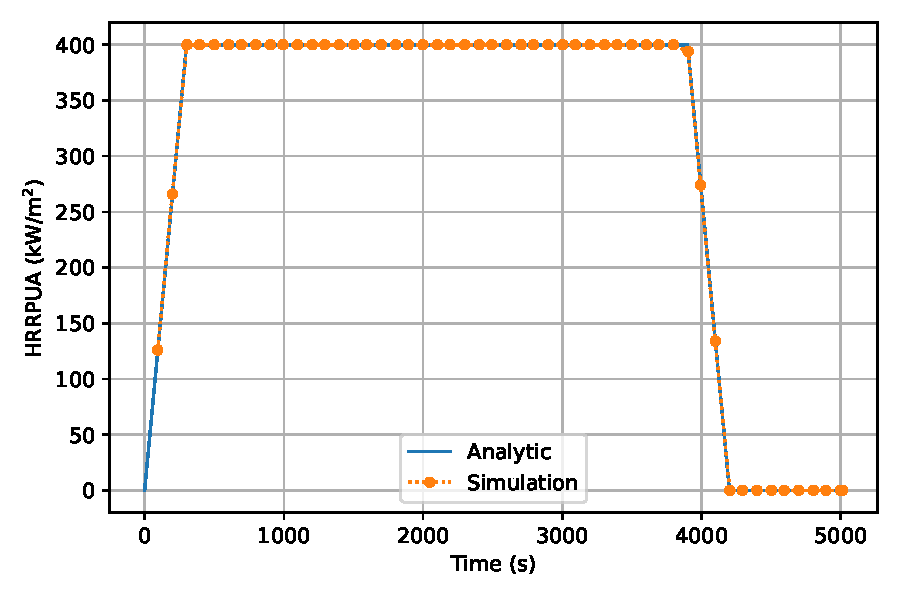
\includegraphics[width=0.7\textwidth]{../figures/hrr_history.pdf}
  \caption{Transient HRR (analytic vs. simulation).}
  \label{fig:hrr_history}
\end{figure}

\begin{figure}[h]
  \centering
  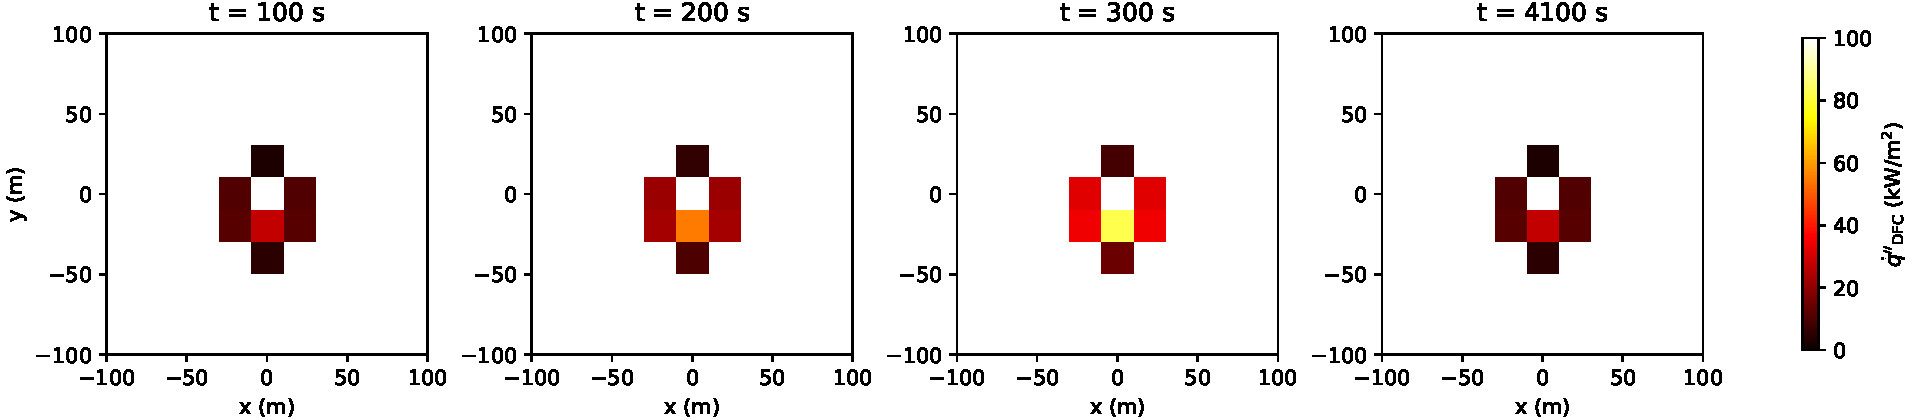
\includegraphics[width=0.95\textwidth]{../figures/dfc_analytic_frames.pdf}
  \caption{Analytic DFC heat flux at selected times.}
  \label{fig:dfc_analytic_frames}
\end{figure}

\begin{figure}[h]
  \centering
  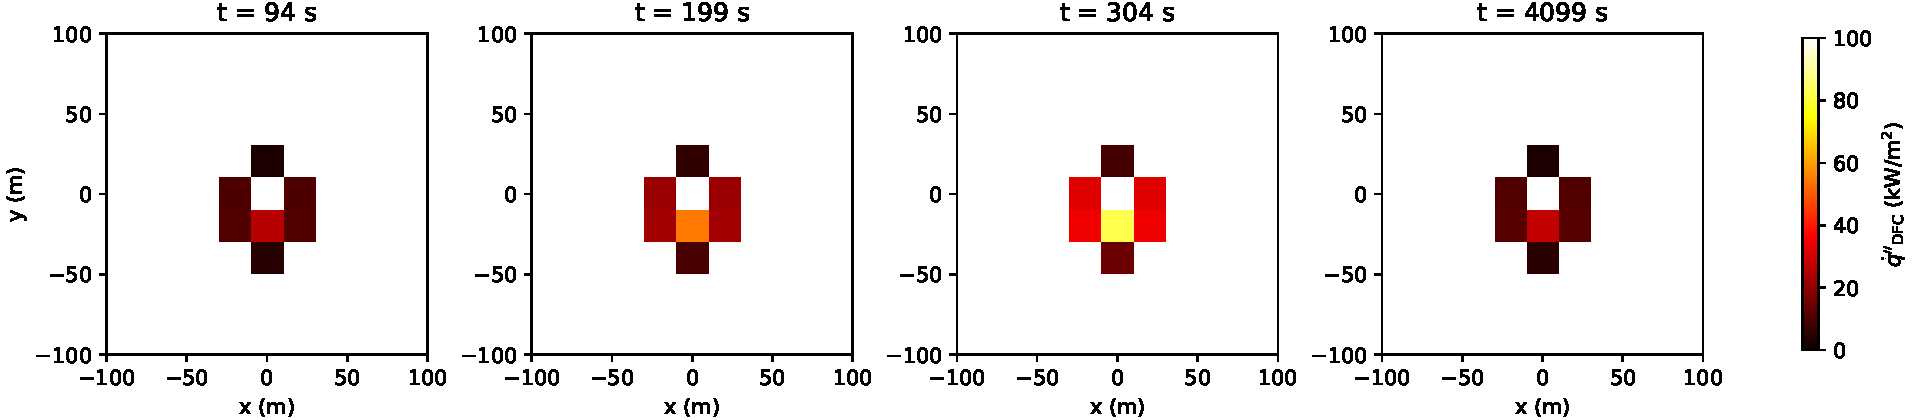
\includegraphics[width=0.95\textwidth]{../figures/dfc_sim_frames.pdf}
  \caption{Simulated DFC heat flux at selected times.}
  \label{fig:dfc_sim_frames}
\end{figure}

\begin{figure}[h]
  \centering
  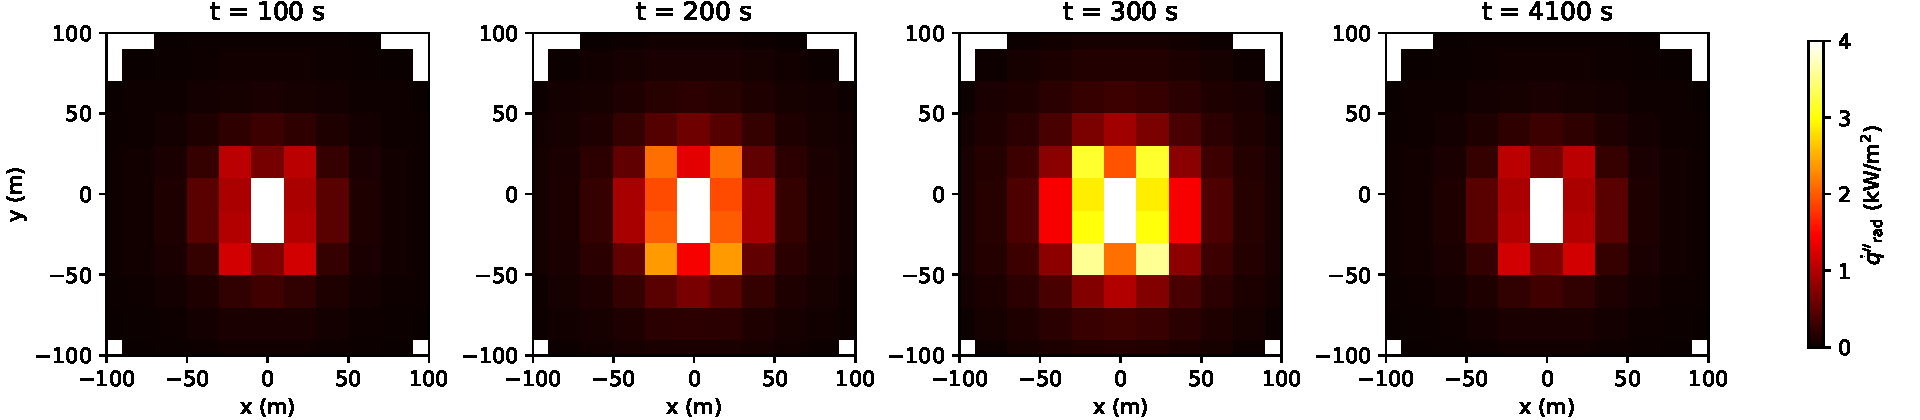
\includegraphics[width=0.95\textwidth]{../figures/rad_analytic_frames.pdf}
  \caption{Analytic radiative heat flux at selected times.}
  \label{fig:rad_analytic_frames}
\end{figure}

\begin{figure}[h]
  \centering
  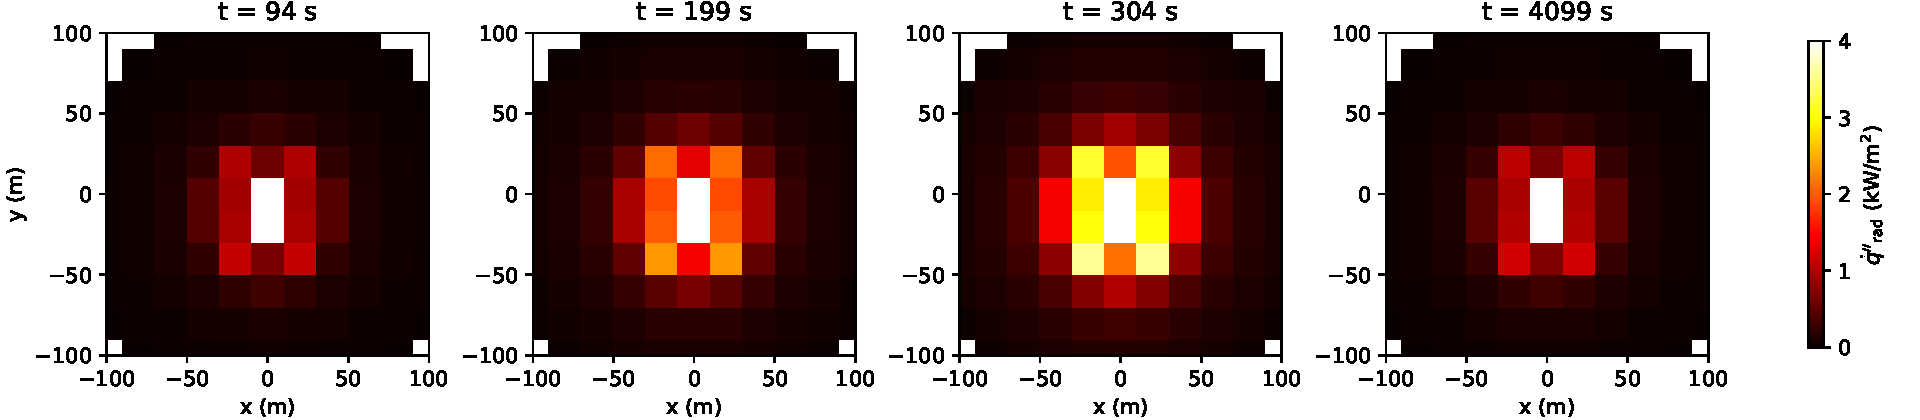
\includegraphics[width=0.95\textwidth]{../figures/rad_sim_frames.pdf}
  \caption{Simulated radiative heat flux at selected times.}
  \label{fig:rad_sim_frames}
\end{figure}

\begin{figure}[h]
  \centering
  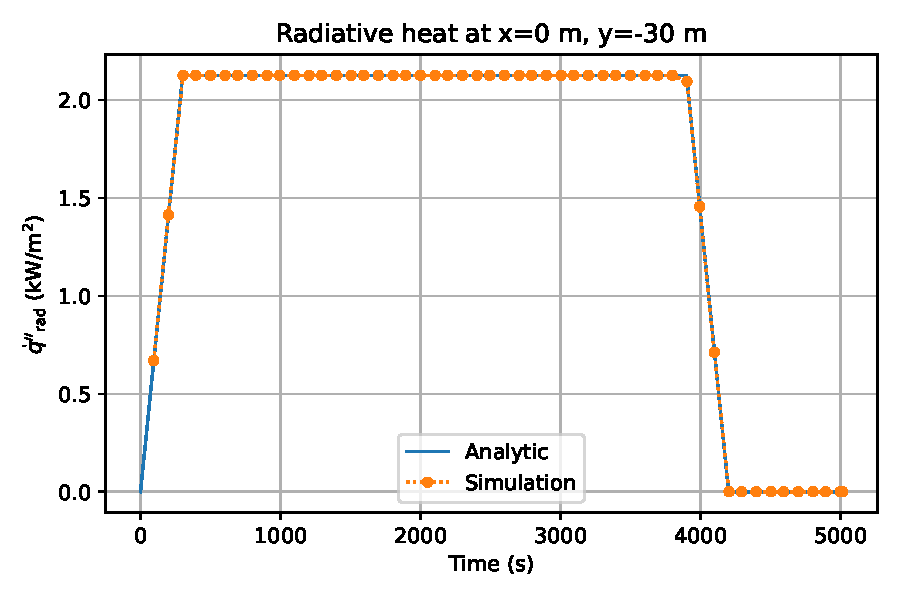
\includegraphics[width=0.7\textwidth]{../figures/rad_history_xy0_m30.pdf}
  \caption{Radiative heat flux time history at $(x,y)=(0,-30)$ m.}
  \label{fig:rad_history_xy0_m30}
\end{figure}

\begin{figure}[h]
  \centering
  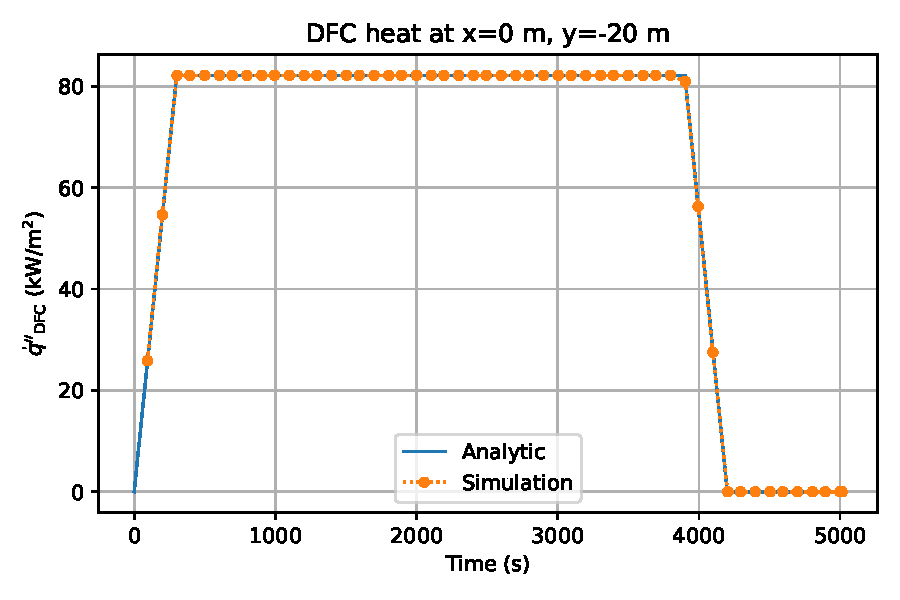
\includegraphics[width=0.7\textwidth]{../figures/dfc_history_xy0_m20.pdf}
  \caption{DFC heat flux time history at $(x,y)=(0,-20)$ m.}
\label{fig:dfc_history_xy0_m20}
\end{figure}


\subsection{Discussion}
\begin{itemize}[nosep]
  \item Clarify parameter sensitivities (e.g., $A,D,W_p$) and wind-direction convention: $\theta_{\mathrm{wind}}=\frac{\pi}{180}(270-\mathrm{WD}_{20ft})$ points the major axis toward $+x$ when $WD_{20ft}=0^\circ$.
  \item Document any discretization effects at coarse $\Delta$ and how $C_\mathrm{HRR}$ compensates for footprint changes.
  \item Note corner cases: $E_{b2}\le 0$ (degenerate $b$), transition regions in the piecewise wind regression, and clipping of coverage fractions.
\end{itemize}

\subsection*{Reproducibility}
\begin{itemize}[nosep]
  \item MATLAB functions: \texttt{ellipse\_ucb}, \texttt{hrr\_transient}, \texttt{heat\_flux\_calc}.
  \item Command(s): \texttt{./run\_case.sh}; environment: \texttt{<modules/conda env>}.
  \item Logs under \texttt{cases/\CaseID/logs/}; figures in \texttt{cases/\CaseID/figures/}.
\end{itemize}

\end{document}
